\chapter{随机变量的数值特征}

\section{期望}

\begin{definition}
    对于实值随机向量$X : (\Omega,\mathscr{F},\P) \to (\R,\mathscr{B}_{\R})$和(可测)函数$g : \Rn \to \R$, 称
    \[ \E[g(X)] = \int_{\Omega} g(X(\omega))\,\d\P(\omega) = \int_{\R} g(x) \,\d F_{X}(x) \]
    为$g(X)$的\textbf{期望}(expectation).
\end{definition}

\begin{remark}
    当$F_{X}(x)$在$x_0$出连续可导时, $\d F_{X}(x_0)=f_{X}(x_0)\d x$; 当$x_0$为其间断点时时, $\d F_{X}(x_0)=p_{X}(x_0)\delta(x_0)\d x$
\end{remark}

期望算子$\E$是一个线性泛函, 仅适用于\underline{可积}的随机变量.

\begin{definition}
    \begin{enumerate}
        \item 当$g(x)=x$时, $\E[g(x)]=\E[X]$称作$X$的\textbf{均值}(mean), 记为$\mu_{X}$
        \item 当$g(x)=(x-\mu_{X})^{2}$时, $\E[g(x)]=\E[(X-\E[X])^{2}]$称作$X$的\textbf{方差}(variance), 记为$\sigma^2_{X}$. 其平方根称作$X$的\textbf{标准差}(standard deviation), 记为$\sigma_{X}$
        \item 当$g(x,y)=(x-\mu_{X})(y-\mu_{Y})$时, $\E[g(X,Y)]=\E[(X-\E[X])(Y-\E[Y])]$称作$X$与$Y$的\textbf{协方差}(covariance), 记为$\Cov(X,Y)$或$\sigma_{XY}$.
        \item 定义$X$与$Y$的\textbf{相关系数}(correlation coefficient)为:$\sigma_{XY}/(\sigma_{X}\sigma_{Y})$, 记为$\Cor(X,Y)$或$\rho_{XY}$. 若$\rho_{XY}=0$, 则称$X$与$Y$不相关
    \end{enumerate}
\end{definition}

\subsection{均值}

\begin{remark}
    \begin{itemize}
        \item 随机变量的均值可看作其加权平均, 权重为其pdf或pmf, 也即其质心. 从大数定律(\ref{chap:limitation})的角度看, 也可解释为其长期均值.
        \item 方差为随机变量距其均值的均方偏差, 刻画了$X$的变动程度
        \item 随机变量的均值与标准差的单位和其本身的相同, 方差的为其平方
    \end{itemize}
\end{remark}

\begin{theorem}
    均值为随机变量的线性映射, 即:
    \[ \E(a+\sum_{i=1}^n b_i X_i)=a+\sum_{i=1}^n b_i\E( X_i) \]
\end{theorem}

\begin{theorem}[]
    若$X,Y$独立,则
    \begin{gather*}
        \E(XY)=\E(X)\E(Y)
        \E(g(X)h(Y))=\E(g(X))\E(h(Y))
    \end{gather*}
\end{theorem}

\begin{remark}
    由于$\E(X/Y)= \E(X)\E(\frac{1}{Y})$, 而$\E(\frac{1}{Y}) \neq \frac{1}{\E(Y)}$, 所以$\E(X/Y)\neq \E(X)/\E(Y)$
\end{remark}

\begin{theorem}
    若$g$为\underline{下凸(convex)函数}, 则$\E[g(X)] \ge g[\E(X)]$; 若$g$为\underline{上凸(concave)函数}, 则$\E[g(X)] \le  g[\E(X)]$;
\end{theorem}

\begin{figure}
    \centering
    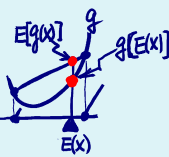
\includegraphics{image/trans_mean.png}
\end{figure}

一个重要结果是, 若$g(X) \ge 0$, 则$\E[g(X)] = 0 \implies g(X) \overset{\as}{=} 0$, 即$\P\{g(X)=0\} = 1$. 其证明可通过\textbf{Markov不等式}
\[ \P\{g(X)\ge\e\} \le \E[g(X)]/\e, \quad \forall \e > 0 \]
完成, 其中需要用到概率的\emph{连续性}, 即$\lim\limits_{n\to\infty}A_{n} = A \implies \lim\limits_{n\to\infty}\P(A_{n}) = \P(A)$.

预处理随机变量有两个常用变换:
\begin{itemize}
    \item \textbf{中心化}(centralization) $X \mapsto X-\E{X}$;
    \item \textbf{标准化}(standardization) $X \mapsto \dfrac{X-\E{X}}{\sqrt{\Var(X)}}$.
\end{itemize}

\subsection{方差}

\begin{theorem}
    $\sigma^2_X=\operatorname{Var}(X)=\E[(X-\mu_X)^2]=E(X^2)-\mu_X$
\end{theorem}

\begin{theorem}
    \[ \operatorname{Var}(a+bX)=b^2\operatorname{Var}(X) \]
\end{theorem}

\begin{theorem}
    \[ \operatorname{Var}(a+\sum_{i=1}^n b_i X_i)=\sum_{i=1}^n b_i^2 \operatorname{Var}(X_i)+\mathbf{b}^{\mathrm{T}} \Sigma \mathbf{b}\]
    其中$\Sigma$为协方差矩阵, $\Sigma_{i,j}=\operatorname{Cov}(X_i,X_j)$
\end{theorem}

\begin{theorem}
    若$X_1,\cdots ,X_n$相互独立, 则:
    \[ \operatorname{Var}(\sum_{i=1}^n X_i)=\sum_{i=1}^n\operatorname{Var}( X_i) \]
\end{theorem}

考虑\textbf{均方误差}(mean squared error)
\[ \MSE(X;\theta) = \E[|X-\theta|^{2}], \quad \theta\in\R, \]
通过\textbf{方差偏差分解}(variance-bias decomposition)
\[ \MSE(X;\theta) = \Var(X) + |\E{X}-\theta|^{2} \]
可以说明$\theta\mapsto\MSE(X;\theta)$在$\E{X}$处取到最小值$\Var(X)$.

\emph{投影}(projection)和\emph{正交分解}的思想在各种内积空间中应用广泛, 这里是$\E = \proj{}{\R}$, 概率论中关于子事件域$\mathscr{G}$ (随机元$X$, resp.)的\emph{条件期望}几何直观是$\proj{}{\mathscr{G}}$ ($\proj{}{\sigma(X)}$, resp.), 线性模型$\mathbf{y} = \mathbf{X}\bm{\beta} + \bm{\e}$中\emph{拟合值}为$\hat{\mathbf{y}} = \proj{\mathbf{y}}{\operatorname{Col}(\mathbf{X})}$.

\begin{theorem}[Chebyshev不等式]
    设随机变量$X$的均值与方差分别为:$\mu, \sigma^2$, 则:
    \[ \P(\left| X-\mu \right| >t)\le \frac{\sigma^{2}}{t^{2}} \]
\end{theorem}

\begin{proof}
    设$f(x)$为$X$的概率密度函数, 令$R=\left\{ x:|x-\mu|>t \right\} $
    \begin{align*}
        \P(|x-\mu|>t) & = \int_R 1 \cdot  f(x)\d x \le \int_R \frac{(x-\mu)^2}{t^{2}}f(x) \d x \\
                      & \le \int_{-\infty}^{\infty}\frac{(x-\mu)^2}{t^{2}}f(x) \d x            \\
                      & = \frac{\sigma^{2}}{t^{2}}
    \end{align*}
\end{proof}

\begin{remark}
    若令$t=k\sigma$, 则$\P(\left| X-\mu \right| >k\sigma)\le \frac{1}{k^{2}}$, 即标准差可代表随机变量偏离均值的概率单位距离.
\end{remark}

\begin{corollary}
    \[ \operatorname{Var}(X)=0 \implies P(X=\mu)=1 \]
\end{corollary}

\subsection{协方差}

协方差代表了$X$与$Y$之间的联合变化倾向, 或者说他们间的相关程度, 但其间\underline{未必有}因果关系.

\begin{theorem}
    \[ \operatorname{Cov} (X,Y)=\E[(X-\mu_X)(Y-\mu_Y)]=\E(XY)-\mu_Y \mu_Y \]
\end{theorem}

\begin{theorem}
    \[ \operatorname{Cov}(a+\sum_{i=1}^n b_i X_i,c+\sum_{j=1}^m d_j Y_j) = \sum_{i=1}^n\sum_{j=1}^m b_i d_j \operatorname{Cov}(X_i,Y_i) = \mathbf{b}^{\mathrm{T}}\Sigma \mathbf{d}\]
\end{theorem}

\begin{theorem}
    独立是不相关的\textbf{充分条件}, 但不是必要条件
\end{theorem}

\begin{theorem}
    $-1\le \rho_{XY} \le 1$, 当且仅当$X$与$Y$间为线性关系时取等号
\end{theorem}

\begin{proof}
    %TODO
\end{proof}

\begin{theorem}
    平移与缩放随机变量都不影响其协方差, 即:
    \[ \left| \operatorname{Cov}(a+ b X,c +d Y) \right| = \left| Cor(X,Y) \right|  \]
\end{theorem}

\section{条件期望}

\begin{definition}
    若$h(Y)$在给定$X=x$下的条件分布(定义\ref{def:cond_dist})的数学期望存在,则定义其为\textbf{条件期望}如下:
    \[ E(h(Y)|X=x) =\begin{cases}
            \sum_{y} h(y) p_{Y|X}(y|x),                    & \text{离散情况} \\
            \int_{-\infty}^{+\infty} h(y) f_{Y|X}(y|x) d y & \text{连续情况}
        \end{cases}\]
\end{definition}

\begin{remark}
    条件期望$\E_{Y|X}(Y|x)$是关于给定变量$x$的函数,不随对应变量$Y$本身变动,但其单位与对应变量$Y$相同,可看作一条在$(X,Y)$平面的曲线。
\end{remark}

\begin{theorem}
    若随机变量$X,Y$独立,则:
    \[ \E_{Y|x}(Y|x)=\E_{Y}(Y) \]
\end{theorem}

\begin{proof}
    由\label{thm:indep_cmf}可知,若随机变量$X,Y$独立,则
    \begin{align*}
        p_{Y|X}(y|x)&=p_{Y}(y) \\
        f_{Y|X}(y|x)&=f_{Y}(y)
    \end{align*}
    所以$\E_{Y|x}(Y|x)=\E_{Y}(Y)$
\end{proof}

由直观感受亦可知:若$X,Y$独立,则$X$不通过任何与$Y$相关的信息,其条件期望亦当与原期望相同。

\begin{note}
    令$g(x)=\E(h(Y)|X=x)$,则$g(X)$是随机变量$X$的变换,也是随机变量,记为$\E(h(Y)|X)$
\end{note}

\begin{theorem}[重期望公式]
    \[ \E_X[\E_{Y|X}(h(Y)|X)] = \E_{Y}[h(Y)] \]
\end{theorem}

\begin{proof}
    %TODO
\end{proof}

\begin{theorem}
    联合期望公式:
    \[ E_{X,Y}=E_X E_{Y|X} = E_Y E_{X|Y} \]
    泛化情况:
    \[ E_{X,Y}[h(X,Y)]=E_X E_{Y|X}[h(X,Y)|X] = E_Y E_{X|Y}[h(X,Y)|Y] \]
\end{theorem}

\begin{theorem}[重方差公式]\label{thm:var_dec}
    随机变量$Y$的方差可作如下分解:
    \[ \operatorname{Var}_Y(Y)=\operatorname{Var}_X[E_{Y|X}(Y|X)] + E_X[\operatorname{Var}_{Y|X}(Y|X)] \]
\end{theorem}

\begin{figure*}
    \centering
    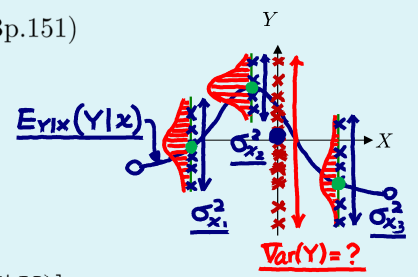
\includegraphics{image/var_dec.png}
\end{figure*}

\begin{corollary}
    \[ \operatorname{Var}_Y(Y) \ge E_X[\operatorname{Var}_{Y|X}(Y|X)] \]
    当且仅当$E_{Y|X}(Y|X)=E_Y(Y)$时取等号
\end{corollary}

\begin{figure*}
    \centering
    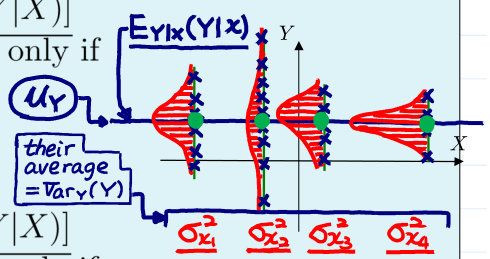
\includegraphics{image/var_dec2.png}
\end{figure*}

\begin{corollary}
    \[ \operatorname{Var}_Y(Y) \ge \operatorname{Var}_X[E_{Y|X}(Y|X)] \]
    当且仅当$\operatorname{Var}_{Y|X}(Y|X)=0$,即$\E_{Y|X}(Y|X)=Y$时取等号
\end{corollary}

\begin{figure*}
    \centering
    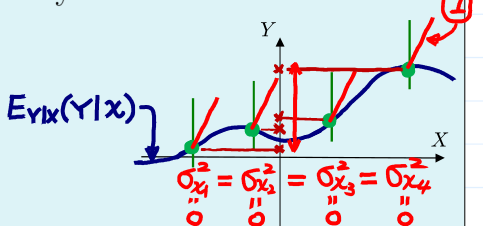
\includegraphics{image/var_dec3.png}
\end{figure*}

\section{矩母函数与特征函数}

\subsection{矩}

\begin{definition}
    对于随机变量$X$, 定义其$k$阶\textbf{矩}(moment)为$E(X^k)$, 记为$\mu_k$; 定义其$k$阶\textbf{中心矩}(central moment)为$E((X-\mu_X)^k)$, 记为$\upsilon_k$;
\end{definition}

易知矩与中心矩间存在以下关系:
\begin{align*}
    \upsilon_k & =\sum_{i=0}^k \binom{k}{i} \mu_i (-\mu_X)^{n-i}     \\
    \mu_k      & =\sum_{i=0}^k \binom{k}{i} \upsilon_i (\mu_X)^{n-i}
\end{align*}

特别的有:
\begin{align*}
    E(X)                  & =\mu_1                                                         \\
    \operatorname{Var}(X) & =\upsilon_2=\mu_1^2-2\mu_1 \cdot \mu_1 + \mu_2 = \mu_2-\mu_1^2
\end{align*}

\subsection{矩母函数}

\begin{definition}
    对于随机变量$X$, 若下式期望存在:
    \[ M_X(t) = \E(e^{tX}) \]
    则称其为\textbf{矩母函数}(moment generating function, mgf)。
\end{definition}

\begin{remark}
    此表达式等价于对概率质量函数或密度函数作Laplace变换, 当$t$取某些特定值时, 可能不存在. (若$t=0$则永远存在)
\end{remark}

\begin{theorem}
    若当$t$属于一个包含零点的开区间时, 矩母函数一直存在, 则其唯一对应一个概率分布.
\end{theorem}

\begin{theorem}
    若当$t$属于一个包含零点的开区间时, 矩母函数一直存在, 则:
    \[ M_X^{(k)}(0) = E(X^k) \]
\end{theorem}

\begin{remark}
    由此可方便地计算各阶矩, 故称其为矩母函数. 反过来, 若已知各阶矩, 通过Tayler展开式$M_X(t)=\sum_{k=0}^{\infty}\frac{M_X^{(k)}(0)}{k!}t^k$还原矩母函数, 进而得出概率分布.
\end{remark}

\begin{proposition}
    若$a,b$为常数, 则
    \[ M_{a+b X}(t) = e^{a t}M_X(b t) \]
\end{proposition}

\begin{theorem}
    若$X,Y$独立,则
    \[ M_{X+Y}(t) = M_X(t) M_Y(t) \]

    泛化情况: 若$X_1,\cdots, X_n$相互独立,则
    \[ M_{X_1+\cdots+ X_n} = \prod_{i=1}^n M_{X_i}(t)\]
\end{theorem}

\subsection{联合特征函数}

\begin{definition}
    对于随机变量$X_1,\cdots, X_n$, 若下式期望存在:
    \[ M_{X_1\cdots X_n}(t_1,\cdots ,t_n) = \E(e^{t_1 X_1+\cdots + t_n X_n}) \]
    则称其为\textbf{联合矩母函数}(joint moment generating function, joint mgf)。
\end{definition}

\begin{remark}
    此处为\underline{多元}函数
\end{remark}

\begin{proposition}
    \[ M_{X_i}(t_i) = M_{X_1\cdots X_n}(0,\cdots ,t_i,\cdots ,0) \]
\end{proposition}

\begin{theorem}
    当且仅当:
    \[ M_{X_1\cdots X_n}(t_1,\cdots ,t_n) = \prod_{i=1}^n M_{X_i}(t_i) \]
    时, $X_1,\cdots, X_n$相互独立
\end{theorem}

\begin{remark}
    与\underline{累计函数、密度函数、质量函数}的情况类似,变量相互独立等价于联合函数可拆分为边缘函数的乘积
\end{remark}

\begin{theorem}
    \[ \frac{\partial^{r_1+\cdots +r_n} }{\partial t_1^{r_1} \cdots  \partial t_n^{r_n}} M_{X_1\cdots X_n}(t_1,\cdots ,t_n) = E(X_1^{r_1} \cdots X_n^{r_n}) \]
\end{theorem}

\subsection{特征函数}

由于有时矩母函数可能不存在,为避免此缺陷,构造出与之特性类似的特征函数。

\begin{definition}
    对于随机变量$X$, 定义其\textbf{特征函数}(characat function, chf)为:
    \[ \phi_X(t) = \E(e^{itX}) = \E(\cos (tX)) + i\E(\sin (tX))\]

    对于随机变量$X_1,\cdots, X_n$, 定义其\textbf{联合特征函数}(joint characat function, joint chf)为:
    \[ \phi_{X_1\cdots X_n}(t_1,\cdots ,t_n) = \E(e^{i (t_1 X_1+\cdots + t_n X_n)}) \]
\end{definition}

\begin{remark}
    此表达式等价于对概率质量函数或密度函数作Fourier变换
\end{remark}

\begin{proposition}
    随机变量的特征函数总是存在
\end{proposition}

\begin{proposition}
    若矩母函数存在,则其与特征函数之间满足关系:
    \[ \phi_X(t) = M_X(it) \]
\end{proposition}

\begin{theorem}
    特征函数可通过以下逆变换得到分布:
    \begin{description}
        \item[离散] $p_{X}(x)=\lim _{T \rightarrow \infty} \int_{-T}^{T} e^{-i t x} \phi_{X}(t) d t$
        \item[连续] $f_{X}(x)=\frac{1}{2 \pi} \int_{-\infty}^{\infty} e^{-i t x} \phi_{X}(t) d t$
    \end{description}
\end{theorem}



\section{熵与信息}
